\documentclass[11pt]{article}
\usepackage[utf8]{inputenc}	% Para caracteres en español
\usepackage{caption}
\usepackage{amsmath,amsthm,amsfonts,amssymb,amscd}
\usepackage{multirow,booktabs}
\usepackage[table]{xcolor}
\usepackage{fullpage}
\usepackage{lastpage}
\usepackage{enumitem}
\usepackage{pgfplots}
\pgfplotsset{compat=1.18}
\usepackage{fancyhdr}
\usepackage{mathrsfs}
\usepackage{wrapfig}
\usepackage{setspace}
\usepackage{calc}
\usepackage{multicol}
\usepackage{cancel}
\usepackage{tikz}
\usetikzlibrary{positioning}
\usepackage[retainorgcmds]{IEEEtrantools}
\usepackage[margin=3cm]{geometry}
\usepackage{amsmath}
\newlength{\tabcont}
\setlength{\parindent}{0.0in}
\setlength{\parskip}{0.05in}
\usepackage{empheq}
\usepackage{framed}
\usepackage[most]{tcolorbox}
\usepackage{xcolor}
\colorlet{shadecolor}{orange!15}
\parindent 0in
\parskip 12pt
\geometry{margin=1in, headsep=0.25in}
\theoremstyle{definition}

\newtheorem{defn}{Definition}
\newtheorem{reg}{Rule}
\newtheorem{exer}{Exercise}
\newtheorem{note}{Note}  % Numbered Note
\newtheorem*{unnote}{Note}  % Unnumbered Note
\begin{document}
\setcounter{section}{0}
\title{Computer Vision Notes}


\thispagestyle{empty}

\begin{center}
{\LARGE \bf Lecture Notes}\\
{\large Computer Vision and Pattern Recognition 8820}\\
Spring 2026
\end{center}
\section{Background}
\subsection{Pinhole Camera and Perspective Foreshortening}
Pin hole camera → approximation (formed at the focal plane of the camera) this doesnt hold true always.

Perspective Projection → used by humans (the model for approximation)
\begin{shaded}

\begin{equation}
\sqrt{
\left(\frac{f x_1}{z} - \frac{f x_2}{z}\right)^2
+
\left(\frac{f y_1}{z} - \frac{f y_2}{z}\right)^2
}
=
\frac{f}{z}
\sqrt{(x_1 - x_2)^2 + (y_1 - y_2)^2}
\end{equation}
\end{shaded}
% \begin{center}
% \parbox{0.9\linewidth}{
% \centering\textit{Perspective foreshortening under a pinhole camera model}
% }
% \end{center}

\noindent
Where, \(f\) is the camera focal length,
\(z\) is the depth of the points from the camera,
and \((x_1,y_1)\), \((x_2,y_2)\) are their coordinates in the camera frame.


% \begin{note}
% \textbf{Capital Letters refer to the accelerating reference frame \textit{S} while lowercase letters refer to the inertial reference frame S$_0$}
% \end{note}
\subsection{Digital Image and Discretisation}
In a 2D sensor (CCD Camera), the image intensity is sampled at discrete points in image plane.
Image plane is discretised into cells and pixels (picture element)

An Image is essentially a 2D array (matrix) of cells and pixels
The pixel coordinates \((i, j)\) refer to center of the cell.
The pixel size essnetialy the image resolution can be measured in terms of pixel per unit area.

Discretisation of the image plane is equivalent to spatial sampling. 

Sampling Density/Resolution Pixels/Unit area

Higher Sampling Density leads to higher image resolution

For a image plane of a given area → smaller pixel size implies higher resolution 
Digital Image → Discretisation of spatial coordinates ( sampling)
\newpage
\textbf{Discretization of intensity values (Quantization)}

Quantization is the discretization of intensity values.

If each pixel is represented using $n$ bits, then the intensity values range from
$0$ to $2^{n} - 1$.
\begin{shaded}
For $n = 8$,
\[
\therefore \text{gray-level intensity values} \in \{0, 1, \ldots, 255\}.
\]
\end{shaded}

% \vspace{0px}

\subsection{Levels of Computation}

\begin{enumerate}
\item \textbf{Pixel Level Computation (contrast enhancement)}
  \begin{itemize}
    \item Output pixel (assume gray scale) Location of pixel or intensity of the pixel (understood in context)
          (spatial and gray scale intensity can mean both)
    \item Each pixel is processed independently
          (parallelism can be applied)
          (massively data parallel operations)
  \end{itemize}

\item \textbf{Local Level Computation (Parallelizable but not easy) (edge)}
  \begin{itemize}
    \item Output Pixel Value = $f(\text{input pixel value, values of pixels in the neighborhood of the input pixel})$
    (overlapping neighbourhood)
  \end{itemize}

\item \textbf{Global Level Computation (distance of gray levels within image)}
  \begin{itemize}
    \item Performed on all pixels in image
    \item Histogram computation
  \end{itemize}

\item \textbf{Object Level Computation}
  \begin{itemize}
    \item This is performed after a semantic entity is extracted from the image (image region)
    \begin{itemize}
      \item Region Size
      \item Region Shape
      \item Region Intensity / Texture
    \end{itemize}
  \end{itemize}
\end{enumerate}

\newpage
\section{Binary Images}
\subsection{Background}
1 pixel → Object Pixel

0 pixel → non object pixel (background pixel)

Shape or Geometry Conveyed (Eg: Silhouette of the person)

Operations on bits (very efficient) (robotic sorting)

How would you create a binary image?

Binary Image (Created by thresholding a gray scale image)

\subsection{Binary Image Formation (Image Taken)}

\[
B(i,j) = \text{threshold}\big(F(i,j)\big)
\]

\[
\text{threshold}\big(F(i,j)\big) =
\begin{cases} 
1, & \text{if } F(i,j) > T \\[2mm]
0, & \text{otherwise}
\end{cases}
\]

\text{\textbf{white objects} against dark background}
\begin{unnote}
\text{Selection of \textbf{T} is based on \textbf{domain knowledge}}
\end{unnote}

\newpage
\section{Geometric Properties of Interests}
\subsection{Object Size}
\begin{unnote}
    Assumption: image contains one object.
\end{unnote}
\begin{enumerate}
    \item Object Size.
    \begin{itemize}
        \item 
        \begin{equation}
        A = \sum_{i=1}^{n} \sum_{j=1}^{m} B(i, j)
        \end{equation}
    \end{itemize}
    \item Centroid
    \begin{itemize}
    \item 
    \begin{equation}
    X_C = \frac{1}{A}\sum_{i=1}^n\sum_{j=1}^m j \cdot B(i,j)
    \end{equation}
    \item 
    \begin{equation}
    Y_C = \frac{1}{A}\sum_{i=1}^n\sum_{j=1}^m i \cdot B(i,j)
    \end{equation}
    \end{itemize}
\item Orientation of Object
\begin{itemize}
    \item Normalising the coordinates based on the centroid
    \[x' =  j -x_c\] 
    \[y' =i-y_c\]
    \item Centralised coordinates wrt to centroid 
    \begin{equation}
    a = \sum_{i=1}^{n} \sum_{j=1}^{m} [x' (i, j)]^2 B(i, j) 
    \end{equation}
\end{itemize}
\end{enumerate}

\section{Moments}
\subsection{Object Orientation}

To compute the second-order moments \( a \), \( b \), and \( c \), we start with the equation:

\[
\tan(2\theta) = \frac{b}{a-c}
\]
\newpage

\begin{shaded}
    \begin{equation}
        a = \sum_{i=1}^{n}\sum_{j=1}^{m}[X^\prime(i,j)]^2 \cdot B(i,j)
    \end{equation}
    \begin{equation}
        b = 2\sum_{i=1}^{n}\sum_{j=1}^{m}[X^\prime(i,j)][Y^\prime(i,j)] \cdot B(i,j)
    \end{equation}
    \begin{equation}
        c = \sum_{i=1}^{n}\sum_{j=1}^{m}[Y^\prime(i,j)]^2 \cdot B(i,j)
    \end{equation}
\end{shaded}
Consider the following expression for \( X^2 \):

\begin{equation}X^2 = \frac{1}{2}(a+c) + \frac{1}{2}(a-c) \cos(2\theta) + \frac{1\cdot b}{2} \sin(2\theta)\end{equation}

Here, \( X^2 \) represents the moment of inertia.

Substitution Step:
Now, we substitute \( 2\theta_1 \) and \( 2\theta_2 \) into the expression for \( X^2 \). The value of \( X^2 \) is minimized for one of them (let's call it \( 2\theta_1 \)) and maximized for the other (denoted as \( 2\theta_2 \)).

Thus, the axis of orientation is the one that minimizes \( X^2 \).

Elongation:
The elongation ratio is given by:

\[
E = \frac{X_{\text{max}}}{X_{\text{min}}}
\]

where \( X_{\text{max}} \) and \( X_{\text{min}} \) are the maximum and minimum moments of inertia.

For a \textbf{sphere} the elongation is:

\[
E = 1
\]

\subsection{Projections}
\begin{equation}
    H[i]  = \sum_{j=1}^{m} B(i, j) 
\end{equation}
\begin{equation}
    V[j]  = \sum_{i=1}^{m} B(i, j)
\end{equation}
Where, H and V are compact representations of $B(i,j)$.



\newpage
\section{Topological Definitions}
\subsection{Path}
A sequence of pixels where successive pixels are neighbours

4 path $\rightarrow$ successive pixels are 4 neighbours 

8 path $\rightarrow$ successive pixels are 8 neighbours

\subsection{Foreground}
The set of pixels with value $1$ denoted by $S$.

\subsection{Connectivity}
A pixel, $p \in S$ connected to pixel  $q\in S$  if there exists a path from p to q consisting entirely of pixels in S (foreground pixels) 

4 connectivity 4 path

8 connectivity 8 path

\subsection{Relations}
\begin{itemize}
    \item p is trivially connected to p (reflexive)
    \item p is connected to q $\Longleftrightarrow$  q is connected to p (symmetric)
    \item if p is connected to q and q is connected to r then p is connected to r (transitive)
\end{itemize}

A subset of pixels on S in which each pixel is connected to all other pixels in the subset.

4 conncected component

8 connected component

The connectivity relation partitions S into connected components

Definition of a partition of a set S into components S1, S2 and S3

\begin{itemize}
\item $S_i = S$
\item $S_i \cap S_j = \phi \forall \text{ i and j}$
\end{itemize}

\newpage
\section{Image Segmentation}
Let $\bar S$  = complement of S

$\bar S =$ set of 0 - pixels $\because S$ is foreground

The set of of all pixels connected components of $\bar S$ that gave some pixels on the image border are referred to as the background.

The other components of $\bar S$  are referred as holes.

Holes are semantically tied to the geometry of the object.

(related to the object)

Background is semantically not related to the object

\subsection{Criteria/Caveat}
\text{Different criteria need to be used for S and $\bar S$ in terms of connectivity}

0 1 0 

1 0 1

0 1 0 

4 4 connected comp in S


$S\prime_{int}$ = $S' - S'_{boundary}$

Surrounded / Contains Relation 

A set of pixels T is  said to be surrounded a set of pixels S if a 4 path from any pixel of S to the image border must intersect T

If T surrounds S then, S is contained in T


\newpage
\section{Connected Component Labelling}
The process by which one assigns a unique label to to each of the connected components 

Components in S

Components in S 

All the pixels within the same component will be assigned the same label
\subsection{Recursive}
\textbf{Recursive CCL Algorithm}
\begin{itemize}
\item Scan the image until an unlabelled 1 pixel is found and assign it a new label L.
\item Assign recursively the label L to all of its neighbouring one pixels…
\item Halt the recursion when no unlabelled 1 pixels are found .
\item Repeat 1 to 3 until no more unlabelled one pixel are found 
\end{itemize}


\begin{unnote}
    Check relation of CCL with flood fill
\end{unnote} 
\subsection{Iterative}

Sequential

\textbf{Iterative CCL Algorithm}

Image Scan

1. Raster Scan (left to right, top to bottom array scan)
2. Serpentine Scan ( lawn mover scan)

*4CC*

1. *Raster scan the image*
2. *If the given pixel p is a 1 pixel*
    1. *if only of u or l has a label then assign that assign label to p*
    2. *Both u and l have the same label then assign that label to p*
    3. *pixel u and l have different labels then assign p the label of u and enter the two labels in an equivalence table*
    4. *Create a new label and assign it to pixel p*
    5. *Continue with the raster scan until no more un-labeled 1 pixel exist.* 
3. *Raster scan the image and for each 1 pixel assign it a single unique label from its equivalence class.*

\newpage
\section{Boundary Extraction}
Binary Image → CCL → Size Filtering

Size Filtering

Replace all components when area < t  with all other 0’ s 

(below the size of smallest object or interests)

 Euler Number

Computed for various objects

E = n.components - n.holes

Boundary Extraction for a Component

1. Perform a raster scan to find the starting pixel of that component 

1. Current pixel $\leftarrow$ starting pixel

b $\longleftarrow$ 4 neighbour to the west of current pixel

1. Enumerate the 8 neighbour of current pixel starting with b in clockwise order. Let these be n1, n2 $\ldots$ n8 (where $n_1$ = b)


1. Determine the smallest i such that $n_i$ belongs to the component

1. Append the current pixel to the contour list (also called a boundary list)
2. Update current $pixel = n_i b \leftarrow n_i-1$
3. Repeat Step 3 to 6 until current pixel comes back to starting pixel 

Boundary Properties

1. Perimeter ( 8 connected )
    1. Trace the boundary list
    2. if the sucessive pixels are 4 neighbours add 1
    3. if the successive pixels are diagonal neighbour add $\sqrt{2}$
2. Compactness of the component
    
    $Compactness = Perimeter^2/Area$
    
    The smaller the compactness the more compact the object
    
    of all 2d shapes the circle has the smallest compactness → 
    
    $$
    Circle = 4\pi^2 r^2 / \pi r^2
    $$
    

\section{Skeletonization of a 2D Shape}

\textbf{Activity Analysis} $\leftrightarrow$ \textbf{Animation}

A 2D shape in the current case is represented as a \emph{binary component}.

\subsection{Distance Measure Properties}

A distance function $d(p,q)$ satisfies the following properties:

\begin{itemize}
\item \textbf{Non-negativity}
\[
d(p,q) \ge 0
\]

\item \textbf{Identity of indiscernibles}
\[
d(p,q) = 0 \iff p = q
\]

\item \textbf{Symmetry}
\[
d(p,q) = d(q,p)
\]

\item \textbf{Triangle inequality}
\[
d(p,r) \le d(p,q) + d(q,r)
\]
\end{itemize}

\subsection{Distance Measures in a 2D Digital Image}

Let
\[
p = (i_1, j_1), \quad q = (i_2, j_2)
\]

\subsubsection{Euclidean Distance}

\[
d_E(p,q) = \sqrt{(i_1 - i_2)^2 + (j_1 - j_2)^2}
\]

\subsubsection{Chessboard Distance}

\[
d_C(p,q) = \max \left( |i_1 - i_2|,\ |j_1 - j_2| \right)
\]


\subsection{Isodistance Contours}

The geometric locust of all points (pixels) that are at a fixed distance from a given point (pixel)

Euclidean distance contour is a circle 

% Manhattan Distance 

% Circle with a square in vertice at top  $D_e = $
\newpage
\section*{Skeletonization Cont.}
The distance transform (DT) of all pixels in component S is the minimum values from the background $\bar S$ for each pixel in S. The distance transform DT image DT(i, j) gives the minimum distance of each pixel (i, j) from $\bar S$.
\subsection{Distance Parallel Algorithm}
\[DT^\circ (i, j) = B(i, j)\]
\[DT^n (i, j) = DT^\circ + min (DT^{n-1}(u,v)\]

(u,v) = set of pixels that $d((i,j), (u, v)) = 1$ unit neighbourhood of (i, j)

d = euclidean, manhattan (u, v) = 4 neighbour of (i, j)

d = chessboard 

(u,v) = 8 neighbours of (i, j)

Check for convergence at end $DT^n (i, j) \neq DT^{n-1}(i, j)$ (hence not converged)
\subsection{Skeleton or the medial axis transform \textit{MAT(i, j)}}
\begin{shaded}
    \begin{equation}
        \text{MAT}(i, j) = \begin{cases}   1, & \text{if } DT(i, j) \geq DT(u, v) \text{ for all } (u, v) \in N(i, j) \\   0, & \text{otherwise} \end{cases}
    \end{equation}
\end{shaded}

\text{MAT}$(i, j) \longleftarrow$ \text{represents the skeleton of the original compound}.\\
Given $MAT (i, j)$ and the $DT$ value for each non zero pixel in $MAT (i, j)$ then one reconstruct the original component (using reverse distance propagation).
\\ \textbf{Halt} when, 
\begin{shaded}
    \begin{equation}
        DT (i, j) = DT(i, j) ^{n-1} \ \forall \text{ i, j}
    \end{equation}
\end{shaded}
\newpage

\section{Region Analysis in Grayscale Images}

\subsection{Formal Definition of image segmentation }
Given an image I, compute a partition $R_1, R_2,...,R_n $ such that,

\begin{shaded}
    \begin{equation}
        \bigcup_{i=1}^{n} R_i - \text{exhaustive}
    \end{equation}
    \begin{equation}
        R_i \cap R_j = \phi \text{ if i and j } -\text{ mutually exclusive/nonoverlapping}
    \end{equation}
\end{shaded}
    
Let $P$ be a predicate that incorporates some homogeneity notion

\begin{shaded}
    \begin{equation}
        P(R_i) = 1 
    \end{equation}
    \begin{equation}
        P(R_i \cup R_j) = 0 \text{ for i } \neq \text{ j}  
    \end{equation}
\end{shaded}

\begin{itemize}
    \item The optimum partition is one for which n is the minimum. (partition into fewest regions) 
    \item Homogeneity criteria needs to be quantified
\end{itemize}


    
\subsection{Image Segmentation (Semantic Image Segmentation)}
Partition the image into regions that correspond to distinct objects

Assign semantic label to each region - semantic segmentation

Two Approaches
\begin{enumerate}
    \item Region based segmentation ( similarity)
    \begin{itemize}
        \item Group together or cluster all pixels that belong to a single object - clustering
    \end{itemize}
    \item Edge Based Segmentation (dissimilarity)
    \begin{itemize}
        \item Detect edge pixels and construct region boundaries or region contours and identify regions - edge detector
    \end{itemize}
\end{enumerate}

\newpage
\section{Modal Analysis}
\subsection{Iterative Threshold Selection}
\begin{itemize}
\item  Determine an initial estimate for $T$ = avg of intensity values of the pixels in the image.
\item Partition the image into two classes $R_1 \text{ and } R_2$ using $T$.
\item Compute the mean gray levels $\mu_1 \text{ and } \mu_2$  of the pixels in $R_1 \text{ and } R_2$ respectively.
\begin{shaded}
\[T_{new} = \frac{\mu_1 + \mu_2}{2}\]
\end{shaded}
\item If $T_{new} = T$ halt else update $T \longleftarrow T_{new}$ and repeat step 2 to 4
\end{itemize}

\begin{unnote}
    For \textbf{step 4} we can also do 
\end{unnote}

\[\alpha \cdot \mu_1 + \beta \cdot \mu_2\] \text{ where } $\alpha$ \text{ and } $\beta$ are the fraction of pixels in $R_1 \text{ and } R_2$ $(\alpha + \beta) =1$
\subsection{Non-Uniform Background (variable thresholding)}
- Capture the variation in background intensity \\
- Eliminate the variation in background intensity from the pixel values $\longrightarrow$ normalization \\
- Threshold based on normalized pixel values

\textbf{Assumptions}
\begin{enumerate}
\item Variation in background intensity values is systematic.
\item Systematic Variation in background intensity values can be captured by a simple function. bilinear and biquadratic
\item Assume that background pixels dominates the foreground pixels. Number of background pixels exceed the number of foreground pixels which essential employs that variation in image intensity values can be attributed to the variation in background intensity values
\end{enumerate}

\subsection{Bilinear Regression}

\begin{equation}
    \frac{1}{N^2}\sum_{x_i}\sum_{y_i}\vert F(x_i, y_i) - F\prime(x_i, y_i) \vert
\end{equation}
\newpage

Compute the normalized pixel values
$F_n = F(x, y)- F\prime(x, y)$

Map $(F_n)_{min} \ldots F(n)_{max}$  $\implies $ (0, max gray level)

use iterative thresholding to threshold the normalized image
\subsection{Model Fitting}
\begin{equation}F_L(x,y) = Ax + By\end{equation}
\begin{center}
    linear
\end{center}
\begin{equation}Q (x, y)= Ax^2 + Bxy+ Cy^2 + Dx + Ey + F\end{equation}
\begin{center}
    biquadratic
\end{center}
\begin{equation}R(x,y = Ax^3 + Bx^2 + Cxy^2 + Dy^3 + Ex^2 + Fxy + Gy^2 + Hx + Iy + J )\end{equation}
\begin{center}
    bicubic
\end{center}
As the number of coeff increases so does the computational complexity increases.
\begin{enumerate}
    \item Pro's
    \begin{itemize}
        \item Less fitting error (higher fitting accuracy)
    \end{itemize}
    \item Con's
    \begin{itemize}
        \item Computational complexity
        \item overfitting
    \end{itemize}
\end{enumerate}


\newpage
\section{Adaptive thresholding}
\begin{enumerate}
    \item Divivde the image into sub images
    \item Perform thresholding independently in each of subimage (eg iterative thresholding)
    \item Combine the threshold results.
\end{enumerate}

Resulting mosiac image will have inconsistency (artifacts).

\pgfplotsset{compat=1.18}
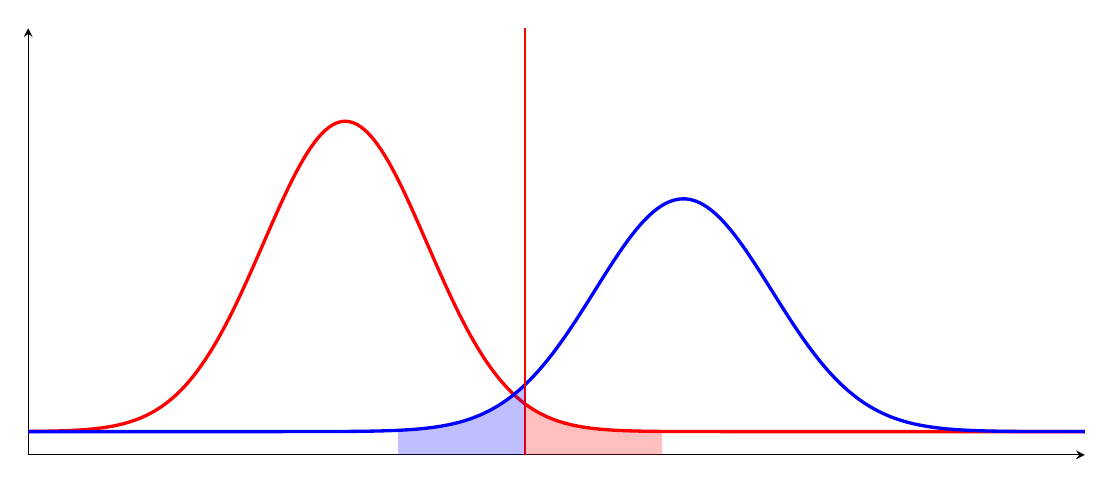
\begin{tikzpicture}
\begin{axis}[
    width=15cm,
    height=7cm,
    xmin=0, xmax=10,
    ymin=0,
    axis lines=left,
    xtick=\empty,
    ytick=\empty,
    samples=300,
    domain=0:10,
]

% --- Red distribution (left, higher)
\addplot[
    red,
    very thick
]
{
    0.12
    + 1.6*exp(-((x-3.0)^2)/1.2)
};

% --- Blue distribution (right, slightly lower)
\addplot[
    blue,
    very thick
]
{
    0.12
    + 1.2*exp(-((x-6.2)^2)/1.4)
};

% --- Decision boundary
\addplot[
    red,
    thick
]
coordinates {(4.7,0) (4.7,2.2)};

% --- Misclassified region (red side)
\addplot[
    red,
    opacity=0.25,
    fill=red,
    draw=none,
    domain=4.7:6.0
]
{
    0.12
    + 1.6*exp(-((x-3.0)^2)/1.2)
} \closedcycle;

% --- Misclassified region (blue side)
\addplot[
    blue,
    opacity=0.25,
    fill=blue,
    draw=none,
    domain=3.5:4.7
]
{
    0.12
    + 1.2*exp(-((x-6.2)^2)/1.4)
} \closedcycle;

\end{axis}
\end{tikzpicture}

\section{Combine histogram with partial information}
\subsection{Dual threhsolding with region growing}
\section*{Algorithm}
\begin{enumerate}
    \item Select threshold $T_1$ and $T_2$
    \item Parititon the image into 3 pixel classes \\
    $R_1 \longleftarrow$ graylevel $\le T_1$ - gaurantee  foreground pixel \\
    $R_2 \longleftarrow$ graylevel $\ge T_2$ - gaurantee  background pixel \\
    $R_3 \longleftarrow$ $T_1 < $\ graylevel $< T_2$ - could be either foreground or background
    \item Visit each pixel in class $R_3$. If the pixel has a neighbour  in class $R_1$ then reassign that pixel to $R_1$
    \item Repeat step 3 until no more $R_3$ pixels are reassigned.
\end{enumerate}

Tries to reduce the \textbf{misclassification} by using spatial coherence

\newpage
\section{Region Representation Schemes}
\begin{unnote}
    Not an Exhuastive List 
\end{unnote}

\begin{enumerate}

    \item \textbf{Array representations}
    
    \begin{itemize}
    
        \item \textbf{Label Array Representation}
        
        \begin{equation}
        L(i, j) = \alpha 
        \text{ if pixel } (i, j) \text{ in image } I(i, j) 
        \text{ has the label } \alpha 
        \text{ belongs to region with label } \alpha
        \end{equation}
        
        
        \item \textbf{Bitmap Representation}
        
        Each label $\alpha$ has an associated bitmap $\beta^{\alpha}$ defined as
        
        \begin{equation}
        \beta^{\alpha}(i,j) =
        \begin{cases}
        1 & \text{if pixel } (i,j) \text{ in image } I \text{ belongs to class } \alpha, \\
        0 & \text{otherwise.}
        \end{cases}
        \end{equation}
        
        The bitmap $\beta^{\alpha}$ is referred to as the \textit{mask} for class $\alpha$.
    
    \end{itemize}

    \item \textbf{Heirarchical Representation} \\
    Represent image and regions at multiple levels of representations.
    \begin{itemize}
        \item Fine analysis at higher resolution (detached)
        \item Coarse Analysis at lower resolution
    \end{itemize}
    
    Only a subset of the image is analyzed at higher resolution - \textbf{Focus of Attention} (FOA) \\
    FOA is Dynamic 
    \begin{itemize}
        \item \textbf{Image Pyramid}
        % \item 
    \end{itemize}
\end{enumerate}

\begin{center}
\begin{tikzpicture}[
    level/.style={draw, minimum width=3cm, minimum height=3cm},
    smalllevel/.style={draw, minimum width=2cm, minimum height=2cm},
    tiny/.style={draw, minimum width=1.4cm, minimum height=1.4cm}
]

% Base
\node[level] (base) at (0,0) {};
\node at (0,-2) {$N = 2^n$};
\node[right=1.2cm of base] {$N$ -- Pyramid base};

% Middle level
\node[smalllevel] (mid) at (0,5) {};
\node[right=1.2cm of mid] {$2^{n-1}$};

% Top level
\node[tiny] (top) at (0,8) {};
\node[right=1.2cm of top] {$2^{n-2} = \dfrac{N}{4}$};

% Vertical arrows
\draw[->, thick] (base.north) -- (mid.south);
\draw[->, thick] (mid.north) -- (top.south);
% \draw[->, thin] (mid.east) -- (mid.west);
% Averaging function
\node at (5,4) (avg) {Averaging function};

\draw[->] (mid.east) -- (avg.west);

% Branch
\node at (9,5) (simple) {simple average};
\node at (9,3) (weighted) {weighted average};

\draw[->] (avg.east) -- (simple.west);
\draw[->] (avg.east) -- (weighted.west);

\end{tikzpicture}
\end{center}


\newpage
\section{QuadTree}
Each node has 4 children or no children (leafnode)

Roof node represents the entire image\\
A leaf node in the quad tree represents homogenous region otherwise the node is split into 4 child nodes
\section*{OctTree}
3-Dimensional representations

\section{Picture tree}
\begin{itemize}
    \item leaf node represent a homogenous region
    \item a non leaf node is split into child nodes based on containment
    \item not a regular structure unlike quad and oct tree
\end{itemize}

\section{Region Adjacency Graph (RAG)}
Scene Graph (RAG is more specialized variant)

\begin{itemize}
    \item Nodes: Represent Regions
    \item Arcs: Represent Common Boundary between two regions
\end{itemize}

\begin{unnote}
    Nodes and Arc possess attribtues
\end{unnote} 
Node Attributes: Region Attributes
\begin{itemize}
    \item Geometric Attributes/Features
    \item Spectral Attributes (avg gray level, texture, color etc \ldots)
\end{itemize}

ARC Attributes: Contour Attributes
\begin{itemize}
    \item 
    \item 
\end{itemize}

\newpage
\section*{RAG Generation}
Given a label array $L(i,j)$ one can generate an RAG
\begin{enumerate}
    \item Raster Scan the L(i,j)
    \item Consider pixel (i,j)
    \begin{itemize}
        \item If node with label L(i,j) exists then update the node in the RAG to include pixel(i, j)
        \item else create a new node with label L(i, j) cosnsiting of pixel (i, j)
    \end{itemize}
    \item Examine the neighbour pixel (i,j)
    \begin{itemize}
        \item if an arc exists between (i, j) and its neighbours region then update it
        \item else create a new arc
    \end{itemize}
    \item Continue with raster scan until all pixels are exhausted
\end{enumerate}


Given the bitmaps $B^\alpha$ (i, j)
\begin{enumerate}
    \item Determine the connected components of $B^\alpha(i,j)$ for each $\alpha$
    \item Create a node for each connected component for all $\alpha$
    \item Trace the boundary of each cc to generate the arcs between the nodes
\end{enumerate}

\section{Over Segmentated Image}
Need to start with a over segemented image because otherwise you will end up improper merge
\ldots

\section{Merge based segementation}

Over segement the image\\
Create initial RAG for the over segemented image\\
visit each node in the RAG\\
a. conside the adjacent nodes\\
b. if the current node and its adjacent node satisfies the merge criteria then merge the nodes and update RAG\\
4. Repeat Step 4 unitl no more merges are possible

\section{Node Selection}
- Random selection of the node\\
- Order the nodes based on same criterion and select the best node
"best" node - longest region (smallest region) \\ 
- list of all pairs of adjacent nodes and select the best pair for merging

\section{Mean Based}
Boundary Contrast Based, Variance Based or Mean Based \\
$\vert \mu_i - \mu_j \vert$

\newpage

% --- Algorithm Parameters ---
\section{Merge Algorithm Parameters}

\begin{itemize}
    \item Selection of nodes for merging
    \item Merge Criterion
    \item Stating point over segemented image
    \item An improper merge cannot be undone
\end{itemize}

\textbf{Split Based Algorithm}

\begin{enumerate}
    \item Start with an initial RAG
    \item Consider a node for splitting
    \item If the node satisfies the split criterion then split it and update RAG
    \item Perform steps 2 and 3 until no more splits are possible
\end{enumerate}

\begin{itemize}
\item Intial RAG - Undersegmented Image
\item Undersegmented Image - Binary Thresholding + CCL
\end{itemize}

\textbf{Splitting Criteria for a node}
\begin{itemize}
    \item Variance test performed in the pixels within the region/component/node
    \item how to split a node
    \begin{itemize}
        \item edge detection within region
        \item contour following
        \item split the region along the contours
        \item split the region along predefined boundary (quad tree)
    \end{itemize}
\end{itemize}

approxmiate the region by fitting to a func 
(homogeneity test) low mean square error then good fit

\section*{Parameters}
\begin{itemize}
    \item splitting criterion
    \begin{itemize}
        \item [-] Variance test 
        \item [-] Function Fitting test (bi linear and quadratic)
    \end{itemize}
    \item Avg Fitting error 
    \item Pixels where fitting error $\gg$ avg fitting error
    \item [-] Candidate along which to split the region
    \item [-] Where to split the region
    \item [-] Node Selection
\end{itemize}

Split where the fit error is higher (not only tells when not to split but also where to split)

\begin{enumerate}
    \item Start with an intial RAG
    \item Go through a split phase
    \item [-] Selecta node that satisfies the split criterion and split it and update RAG.
    \item Merge Phase
    \item [-] Selecta pair of adjacent node
    \item [-] If they satisfy the merge criteria, then merge then and update the RAG
    \item Perform the split and merge phase alternatively
    \item Halt when no more splits or merge are possible
\end{enumerate}

Maintain a list of previously visited k solution states \\
if the current split\/merge results in a previosuly visited stated then reject it and select another node

% tabu list

% \newpage
% \begin{equation}
%     \hat \nabla \mathcal{L} = \frac{\mathcal{L}(\theta + \epsilon\cdot z)-\mathcal{L}(\theta - \epsilon\cdot z)}{\epsilon}
% \end{equation}

\newpage
\section{Iterative Model Fitting (Segementation Technique) with Region Growing}

% Basic Premise 

\subsection*{Basic Premise}

\begin{enumerate}
    \item Segmented image can be modeled as a partition of regions approximated by a parametric function 
    (constant, bilinear, biquadratic, bicubic).

    \item Fitting a function:
    \[
    f = f(x, y, a, m) = \sum_{i+j \le m} a_{ij} x^i y^j
    \]

    \item[] where $x, y$ are variables and $a, m$ are parameters.

    \item For a bilinear fit:
    \[
    f(x, y) = a_{00} + a_{10}x + a_{01}y + a_{20}x^2 + a_{02}y^2 + a_{11}xy
    \]
\end{enumerate}

\subsection*{Fitting Error}

The fitting error over a region $R$ is defined as:

\begin{equation}
X^2(R, a, m) 
= \sum_{(x,y)\in R} 
\left[ F(x, y) - f(x, y, a, m) \right]^2
\end{equation}

\noindent
where $F(x, y)$ is the image intensity function.

\vspace{0.3cm}

For a given region $R$, determine the coefficients $a$ and model order $m$ that minimize the error $X^2$.

% -------------------------------------------------------------------

\section*{Algorithm}

\begin{enumerate}
    \item Determine seed regions in the image — the most homogeneous core of each region.
    
    \begin{itemize}
        \item Use a $5 \times 5$ or $7 \times 7$ window.
        \item Perform a bilinear fit and compute the fitting error.
        \item Select the center of the window where the error is $< T_1$.
    \end{itemize}

    \item For each seed region, perform the following:

    \begin{enumerate}
        \item[(a)] For a given model order, expand the current window (region growing) 
        while keeping the same \underline{\textbf{$a$}} and \underline{\textbf{$m$}}. 
        Compute the fitting error (model extrapolation).
        
        \begin{itemize}
            \item Repeat step (a) until the fitting error $> T_2$.
        \end{itemize}

        \item[(b)] Refit using the same $m$ to obtain a new $a$, then repeat step (a). 
        
        If the refitting error $> T_3$, increase the model order and repeat.

        \item[(c)] Repeat steps (a) and (b) until the maximum model order is reached.
    \end{enumerate}

\end{enumerate}


\end{document}

